\documentclass[crop,tikz]{standalone}
\usepackage{amsmath}
\usetikzlibrary{arrows}
\usetikzlibrary{positioning}
\usetikzlibrary{shapes}
\usepackage[draft]{tikzpeople}

\begin{document}
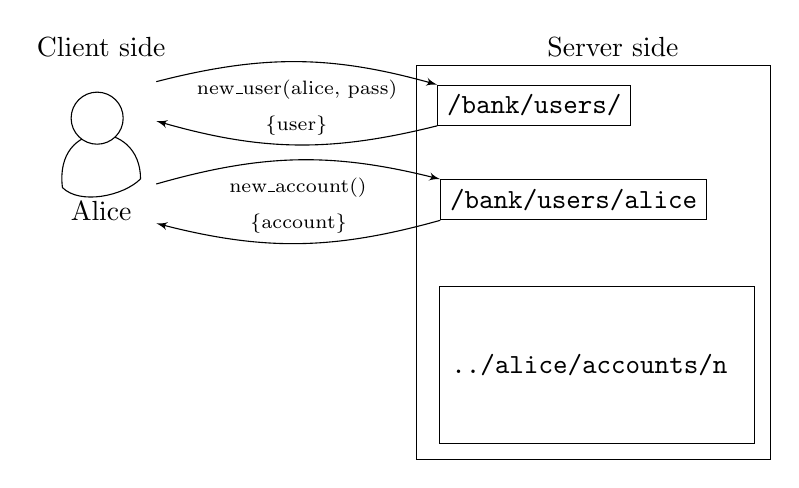
\begin{tikzpicture}
  \tikzset{vertex/.style = {shape=circle,draw,minimum size=1.5em}}
  \tikzset{edge/.style = {->,> = latex'}}
  \tikzset{line/.style={draw, ->, >=latex'}}

  \node[alice,minimum size=1cm] (alice) {Alice} node[above, yshift=1cm]{Client side};
  \draw (4,-4) rectangle +(4.5,5) node[above, xshift=-2cm] {Server side};

  %%%%%%%%%%%%

  \node[draw, align=left] (bu) at (5.5,0.5) {\texttt{/bank/users/}};

  \path (0.7, 0.8) edge[bend left=15, line] node[midway, below,
  yshift=-0.1cm]  {\scriptsize{new\_user(alice, pass)}} (bu.north
  west);

  \path (bu.south west) edge[bend left=15, line] node[midway, above]
  {\scriptsize{\{user\}}} (0.7, 0.3);


  %%%%%%%%%%%

  \node[draw, align=left] (bua) at (6,-0.7)
  {\texttt{/bank/users/alice}};

  \path (0.7,-0.5) edge[bend left=15, line] node[midway, below,
  yshift=-0.1cm]  {\scriptsize{new\_account()}} (bua.north
  west);


  \path (bua.south west) edge[bend left=15, line] node[midway, above]
  {\scriptsize{\{account\}}} (0.7, -1);



  %%%%%%%%%%%

  \node[align=left] (buac) at (6.2,-2.8)
  {\texttt{../alice/accounts/n}};

  \draw (4.3,-3.8) rectangle +(4,2);


\end{tikzpicture}
\end{document}